% Homework report template for courses lectured by Blaz Zupan.
% For more on LaTeX please consult its documentation pages, or
% read tutorials like http://tobi.oetiker.ch/lshort/lshort.pdf.
%
% Use pdflatex to produce a PDF of a report.

\documentclass[a4paper,11pt]{article}
\usepackage{a4wide}
\usepackage{fullpage}
\usepackage[toc,page]{appendix}
\usepackage[pdftex]{graphicx} % for figures
\usepackage{setspace}
\usepackage{color}
\definecolor{light-gray}{gray}{0.95}
\usepackage{listings} % for inclusion of Python code
\usepackage{hyperref}
\renewcommand{\baselinestretch}{1.2}

\lstset{ % style for Python code, improve if needed
language=Python,
basicstyle=\footnotesize,
basicstyle=\ttfamily\footnotesize\setstretch{1},
backgroundcolor=\color{light-gray},
}

\title{Network of Diseases}
\author{Zidar Miha (63060317)}
\date{\today}

\begin{document}

\maketitle

\section{Introduction}


In this homework assignment, we have build a network of deseases, using shared genes for determening connections between them. On top of that network we ran network clustering with label propagation. The key point was to see how and which deseases are connected.

\section{Data}

We were given an OMIM morbidmap file, that contained a list of deseases and their genes. The list of deseases contained multiple lines with the same desease name, so we had to filter the names and join the genes of simmilar names together. By doing that, we have reduced the number of deseases from 6238 to 2448. Because some desease names contain typos, we could reduce the latter number even more if we joined the deseases based on their levinshtein distance. \\

After we build the connected graph, we could see that the degree distribution follows the power law quite nicely (figure: \ref{dd})so we can assume that this graph is Scale free. The graphs are also quite well connected, since the diameter of the largest connected subgraph is only 12. 


\begin{figure}[htbp]
    \begin{center}
        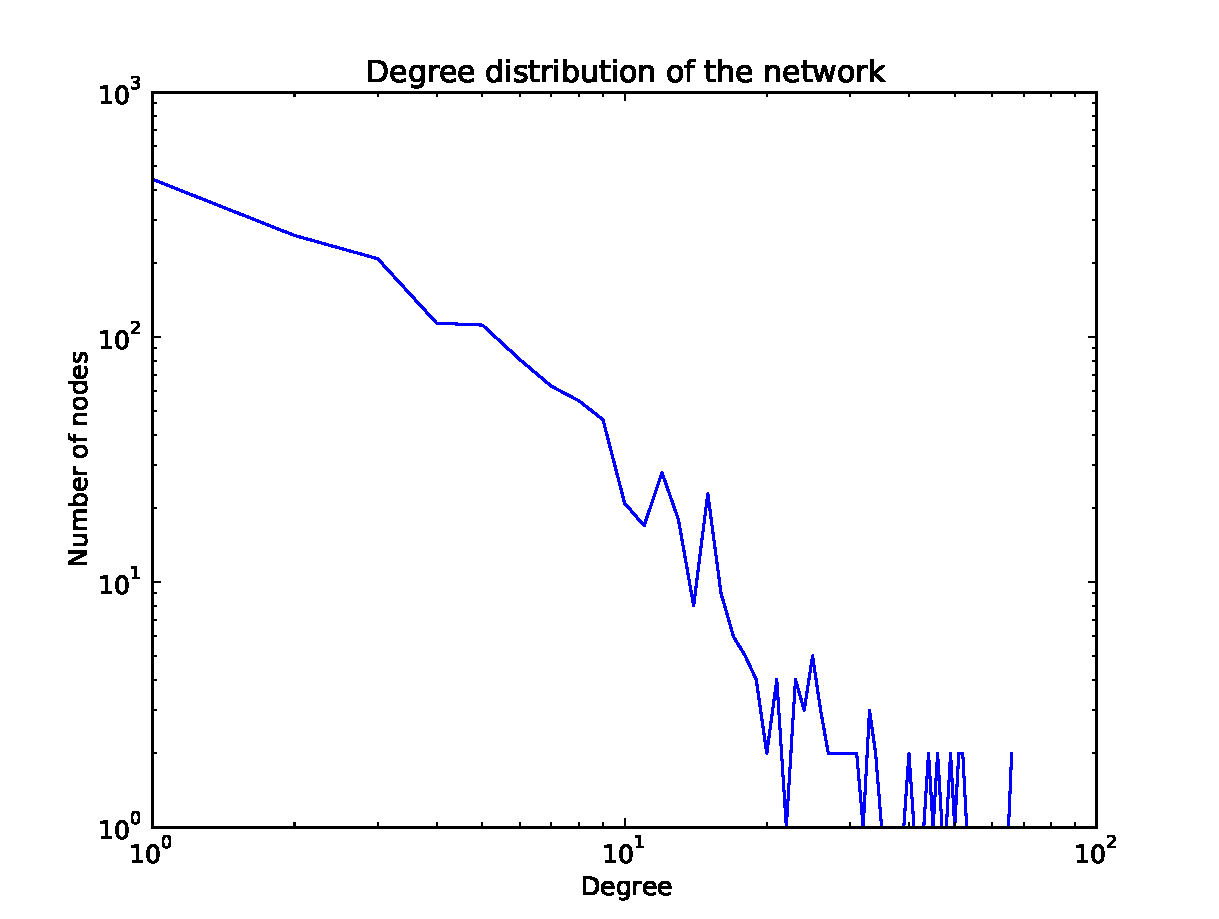
\includegraphics[scale=0.4]{img/ddlog.pdf}
        \caption{Degree Distributiona, in log-log scale}
        \label{ddlog}
    \end{center}
\end{figure}
\begin{figure}[htbp]
    \begin{center}
        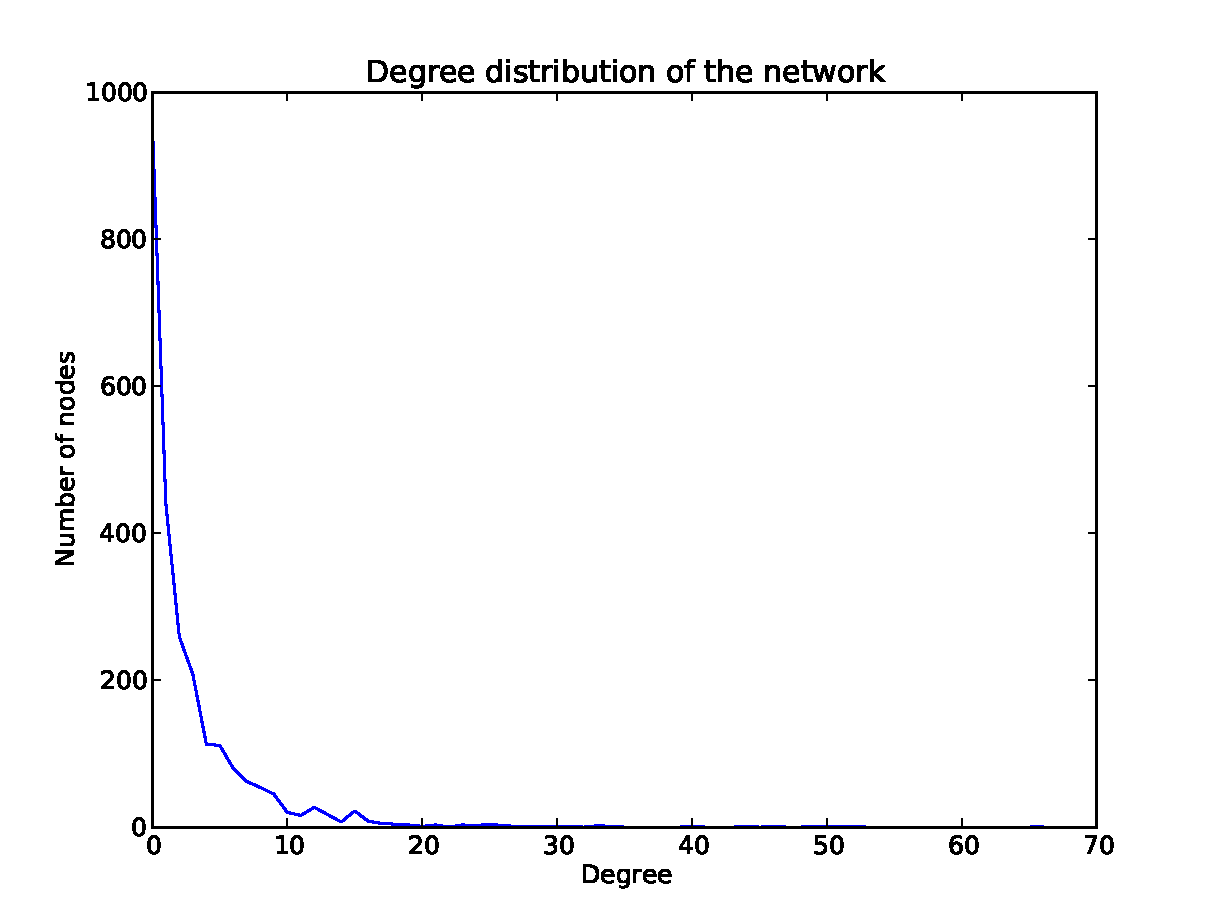
\includegraphics[scale=0.4]{img/dd.pdf}
        \caption{Degree Distributiona}
        \label{dd}
    \end{center}
\end{figure}

\section{Methods}

For clustering we used label propagation algorithm by Raghavan. The algorithm starts with saying that each node is it's own cluster, and then, through a few iterations, it randomly walks over our graph, and updates cluster labels so that each node gets the most common label of its neighbours. If there are more than one such neighbours, then the algorithm should randomly select one of those. The method can run untill the labels are still changing, but I have limited it to a fixed number of iterations. The number of passes we did for the final result was 10000 label updates on the entire graph.

For displaying the graph, we used spring\_layout, implement in pythons networkx librart. That algorithm tries to group the most connected graph points together and kep the distant points away from each other. beacuse this is always just approaching ``the optimal'' layout, it could run forever, so we set a hard limit of 2000 for the final result


\begin{lstlisting}
clusters = {j:i for i,j in enumerate(g.nodes())}
for _ in xrange( iterations ):
    # list of all nodes
    nodes = g.nodes()
    random.shuffle(nodes)
    for node in nodes:
        # count all neigbour labels
        count = labelCounter(g.neighbors(node))
        # select radom candidate from the most common neigbours
        candidate = getCandidate(count)
        clusters[node] = candidate
\end{lstlisting}

\section{Results}

Our full graph has 1110 disjoint subgraphs, most of which are really small, and then we have just one big subgraph with 1118 nodes. The histogram (figure \ref{hist}) shows the distribution of subgraph sizes, without the largest subgraph, because that would obscue the graph too much. \\

Below we have our final resutls of the clustering with the spring layout. Because there are so many nodes, the full view(figure \ref{full}) overlaps too much, we have a smaller slection (figure \ref{izsek}) which shows nice desease groupping.\\

Finally we have extracted clusters in which we have some more known deseases, to inspect what other deseases they relate to. The most surprising relation was between Diabetes, HIV and AIDS (figure \ref{diabetesmellitus3}). \\


\begin{figure}[htbp]
    \begin{center}
        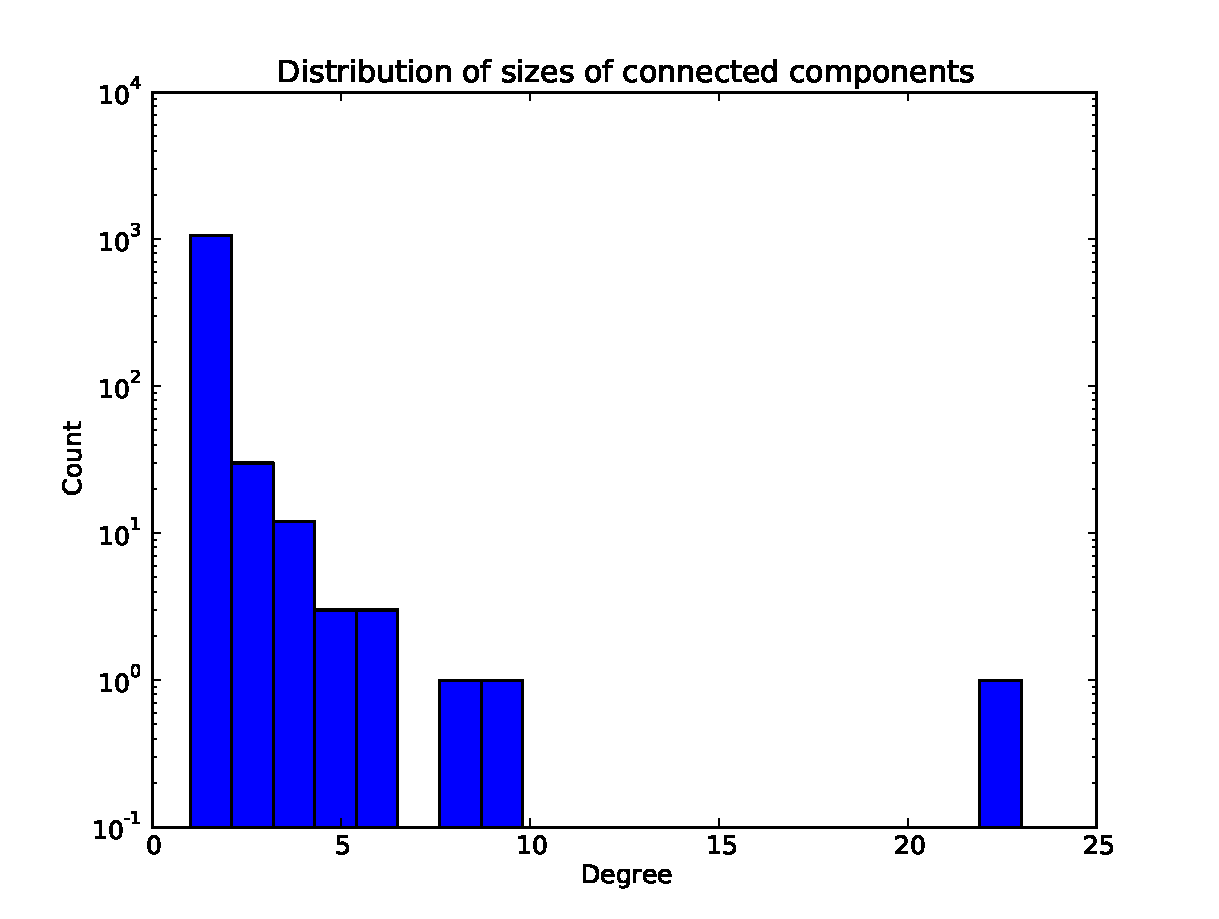
\includegraphics[scale=0.3]{img/dsize.pdf}
        \caption{The distribution of sizes of connected subgraphs}
        \label{hist}
    \end{center}
\end{figure}

\begin{figure}[htbp]
    \begin{center}
        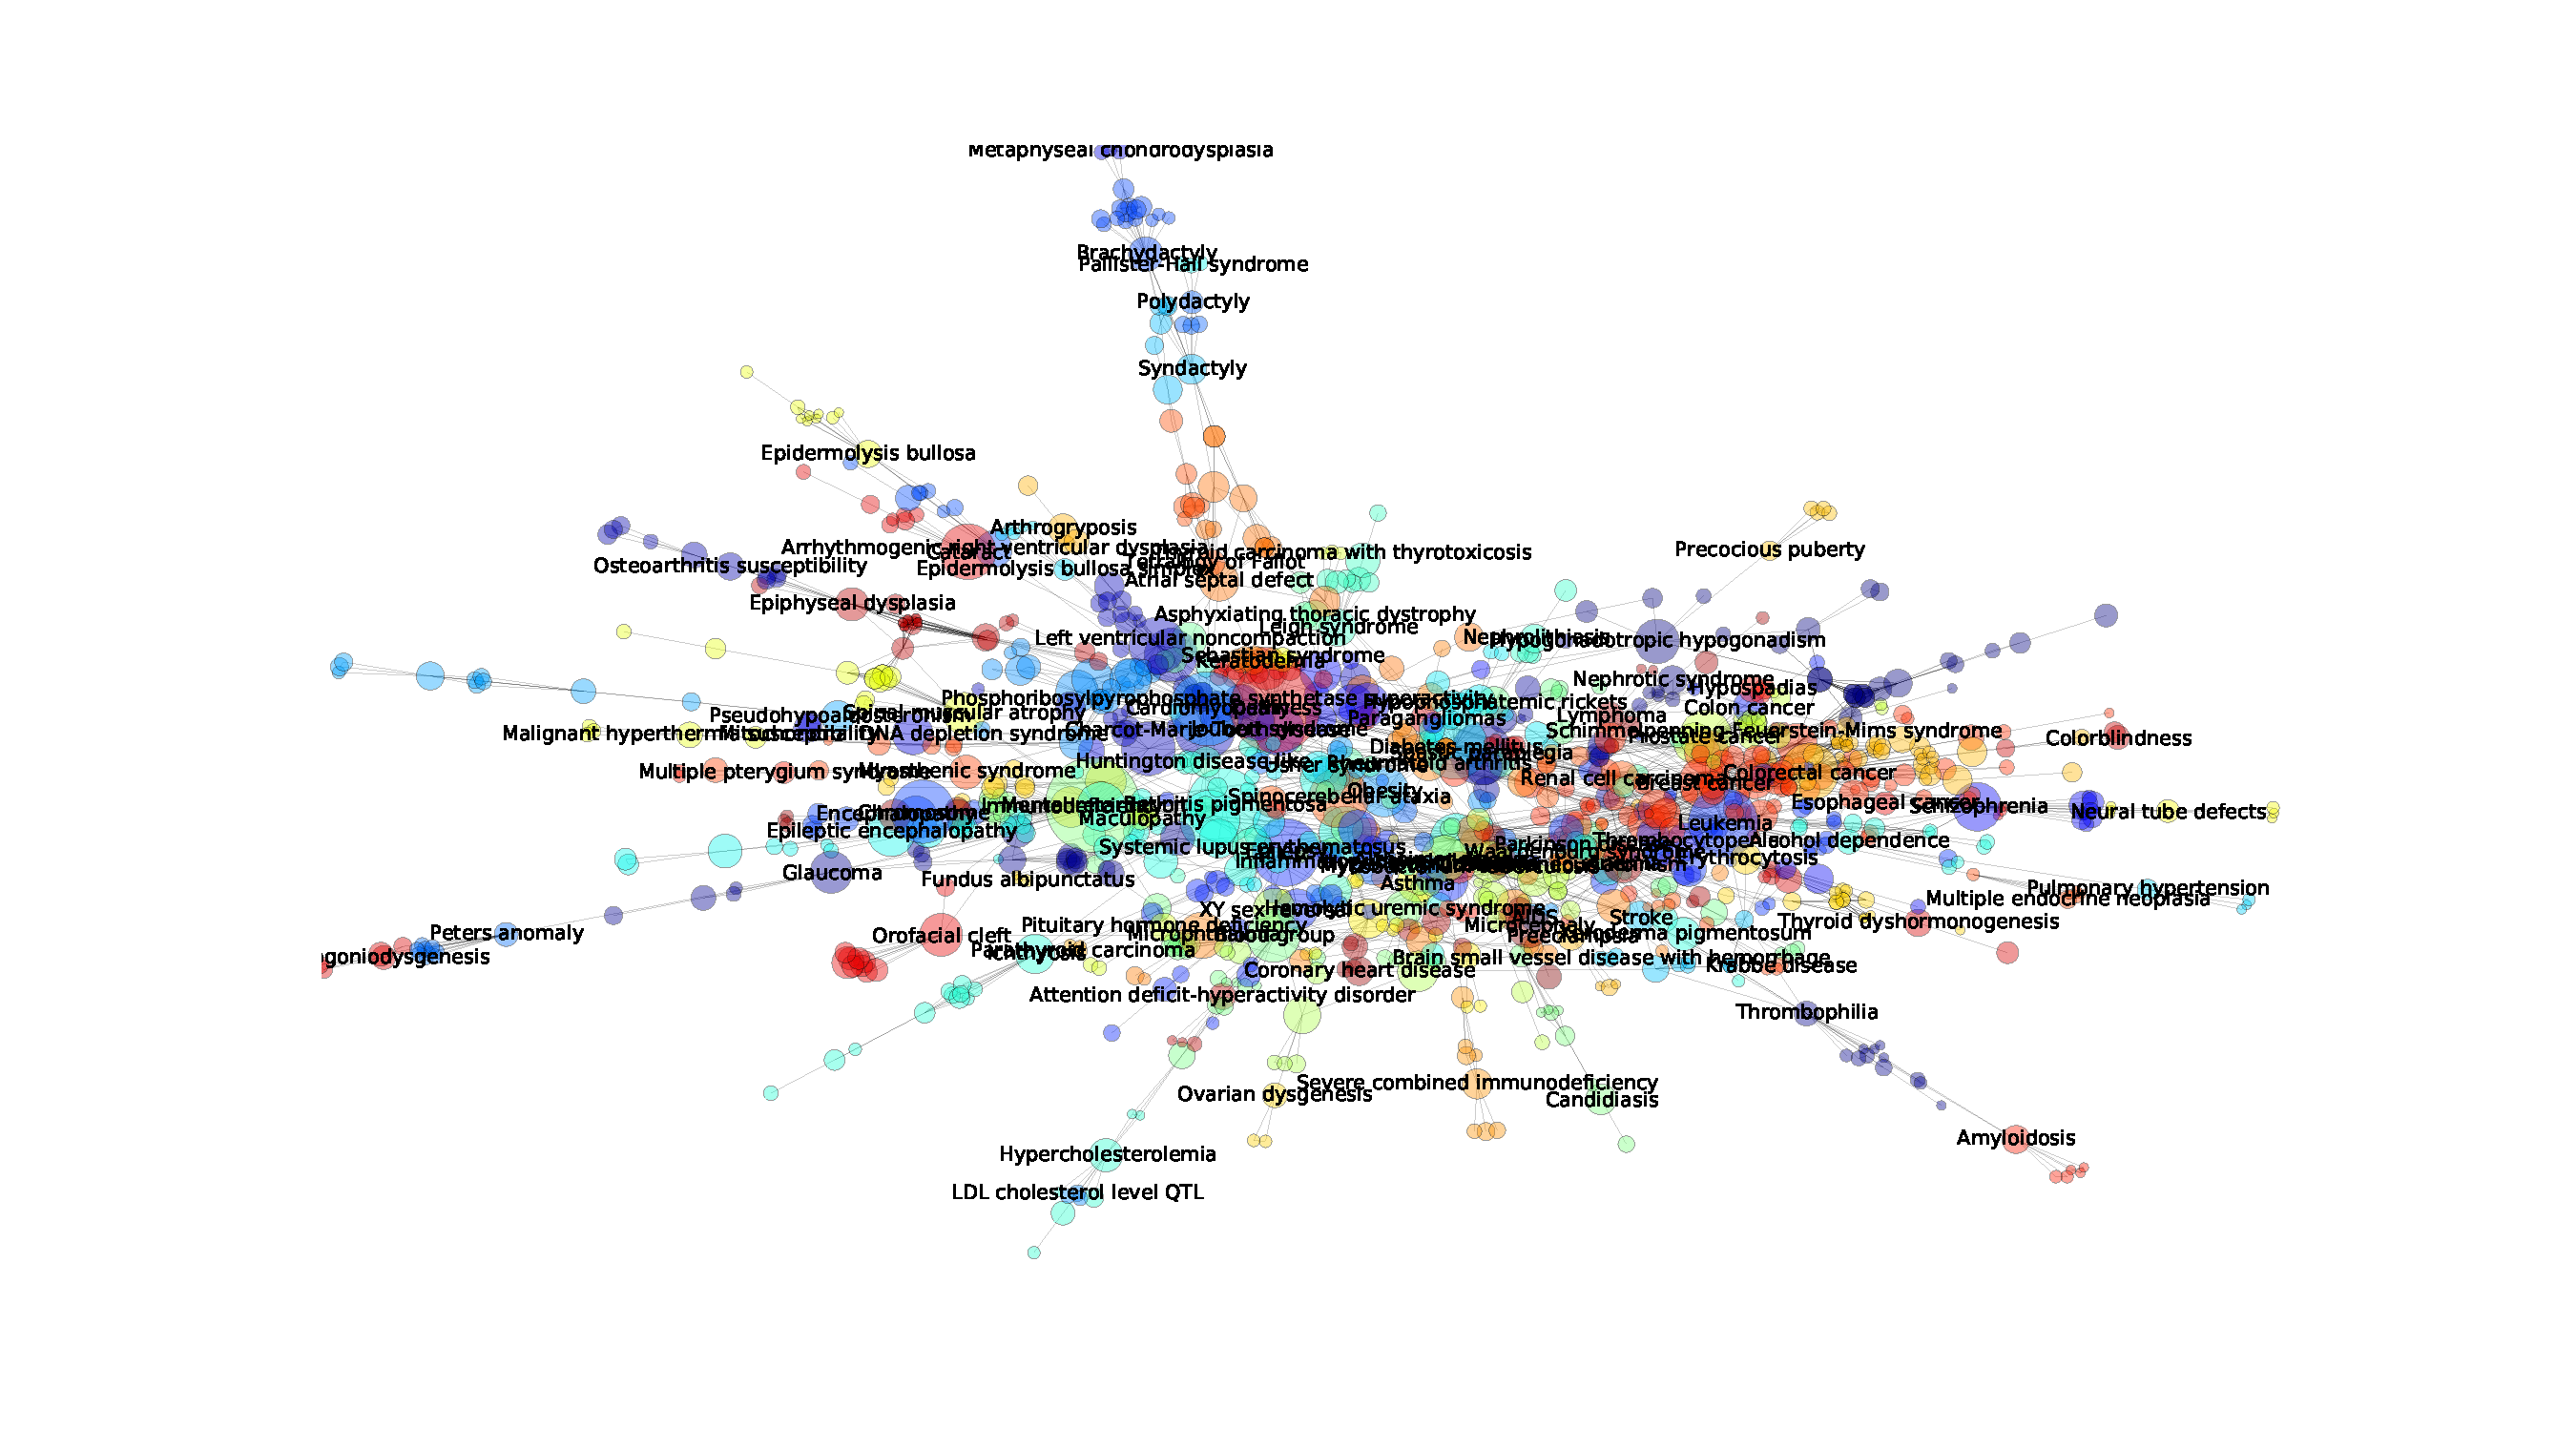
\includegraphics[scale=0.3]{img/full.pdf}
        \caption{Entire graph of teh biggest connected component}
        \label{full}
    \end{center}
\end{figure}


\begin{figure}[htbp]
    \begin{center}
        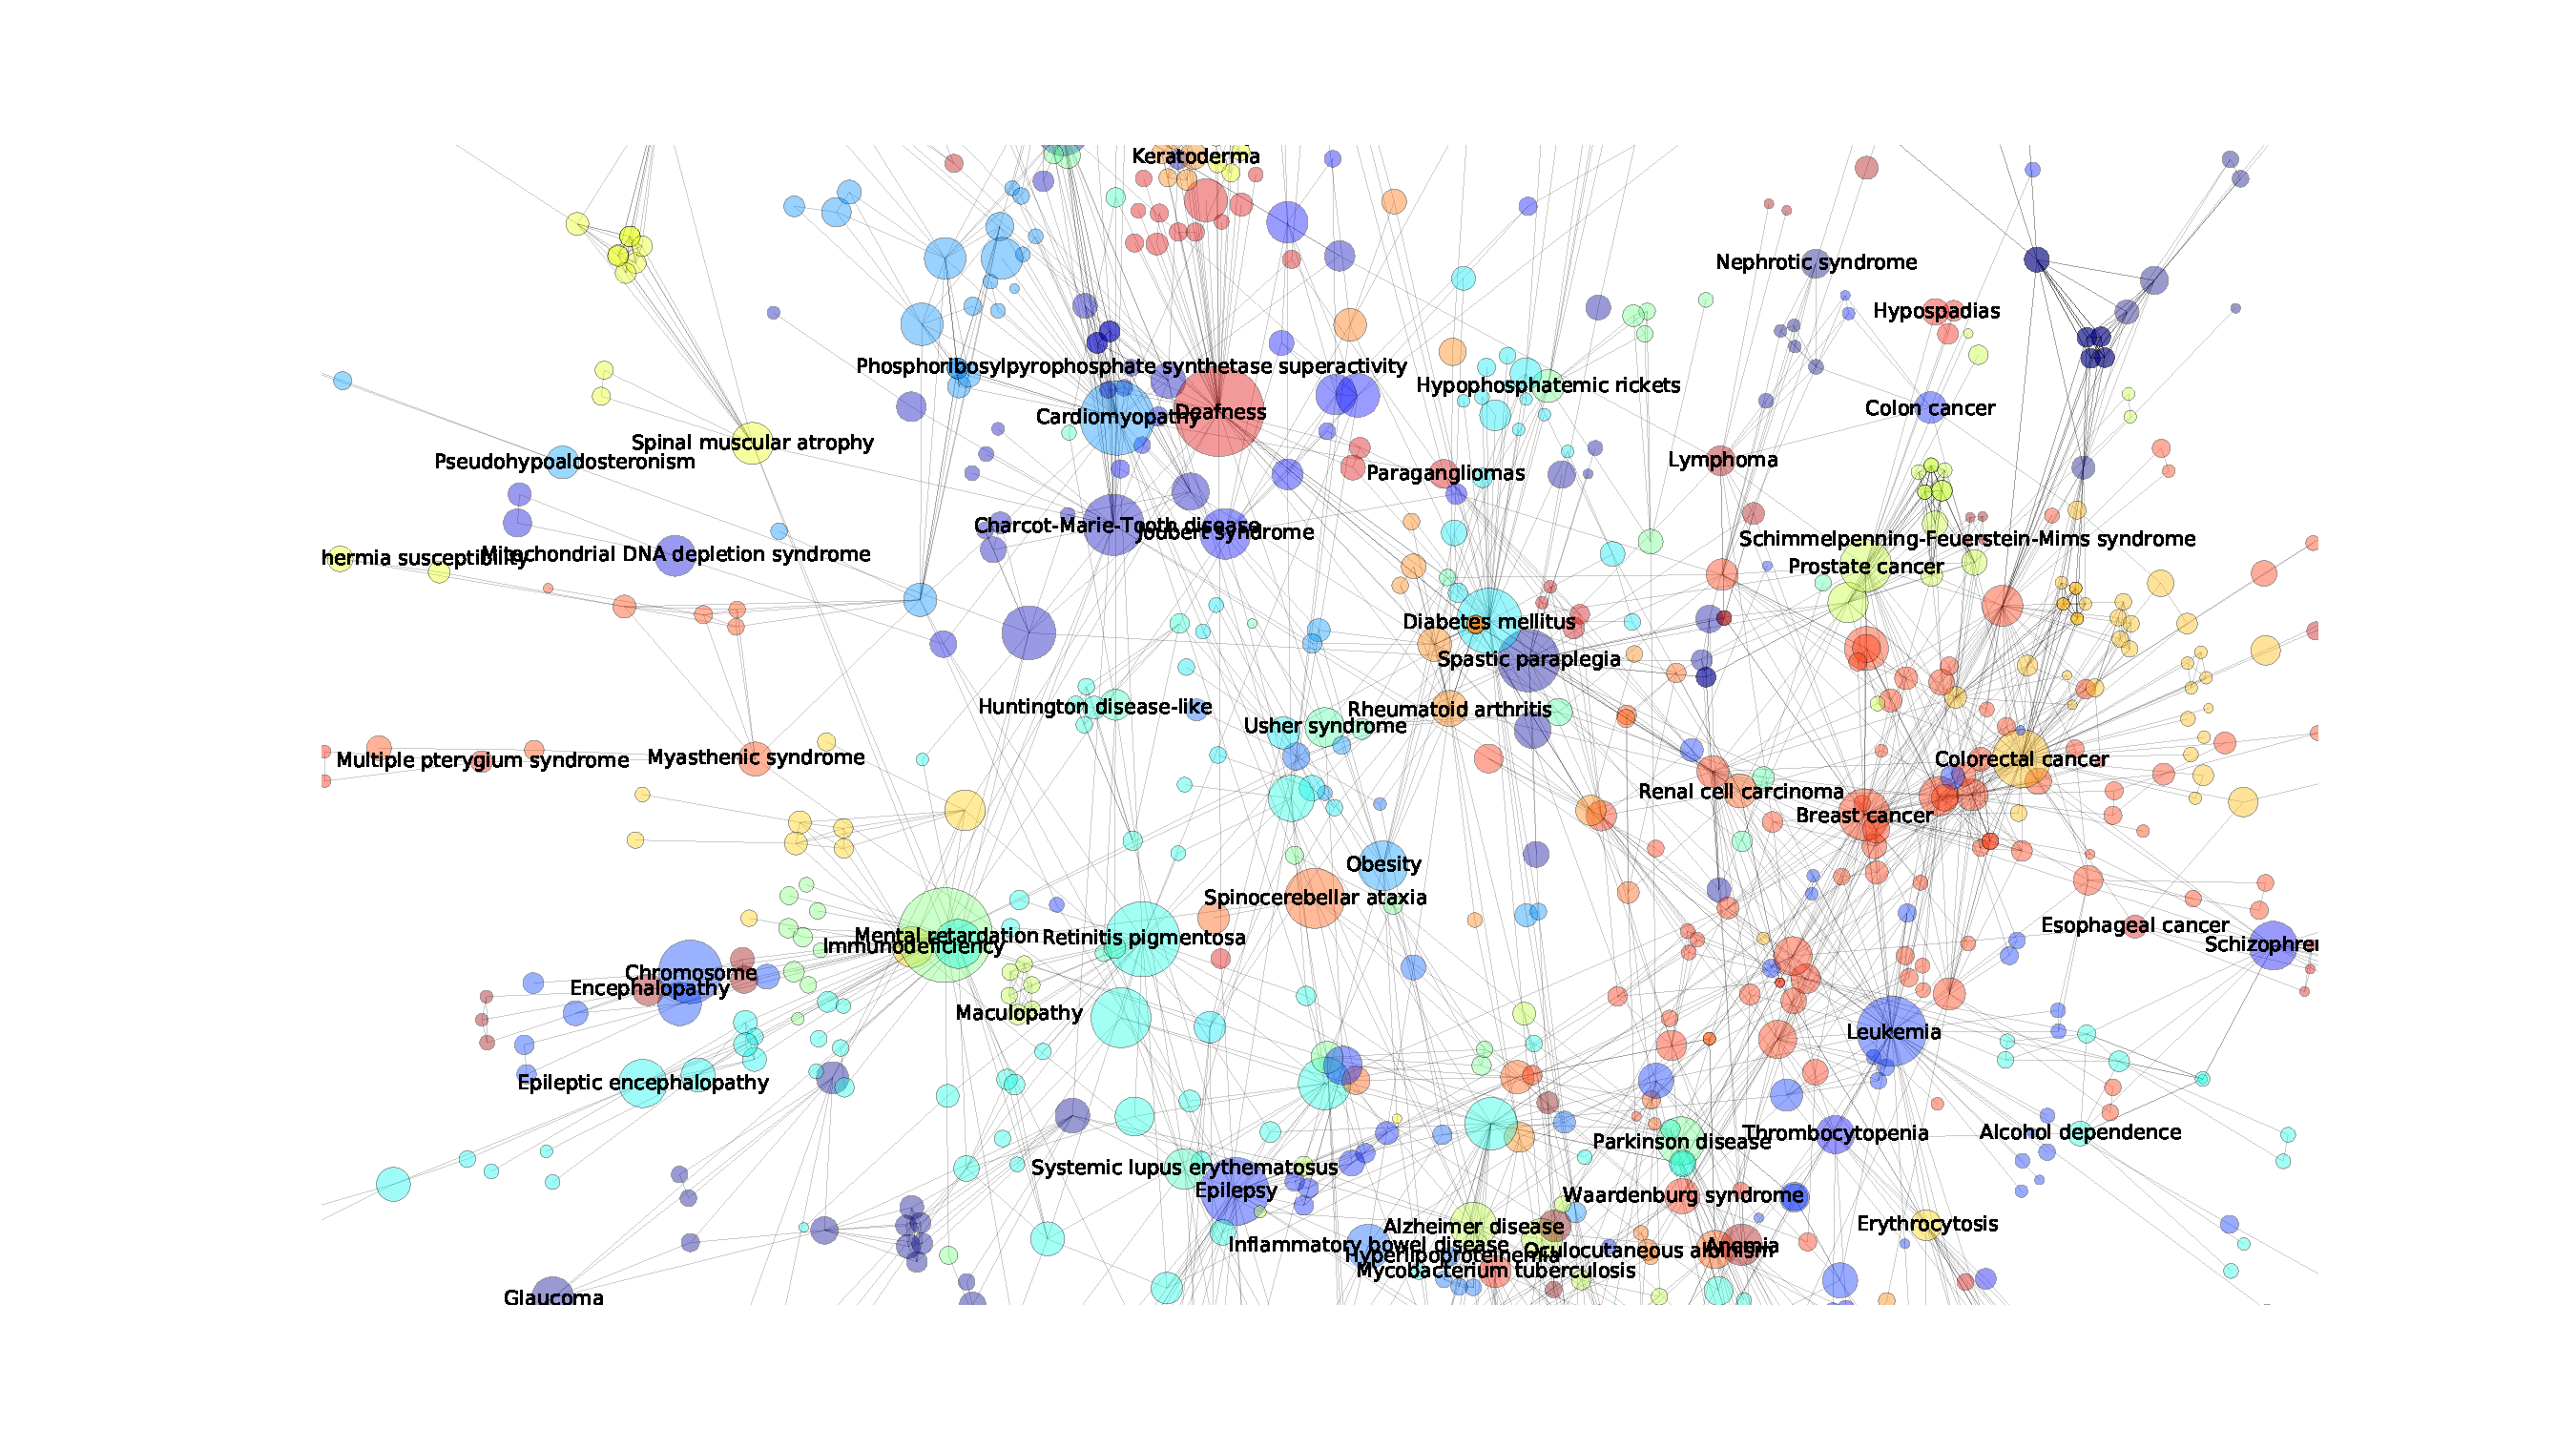
\includegraphics[scale=0.3]{img/izrez.pdf}
        \caption{A smaller section of the graph of teh biggest connected component}
        \label{izsek}
    \end{center}
\end{figure}

\begin{figure}[htbp]
    \begin{center}
        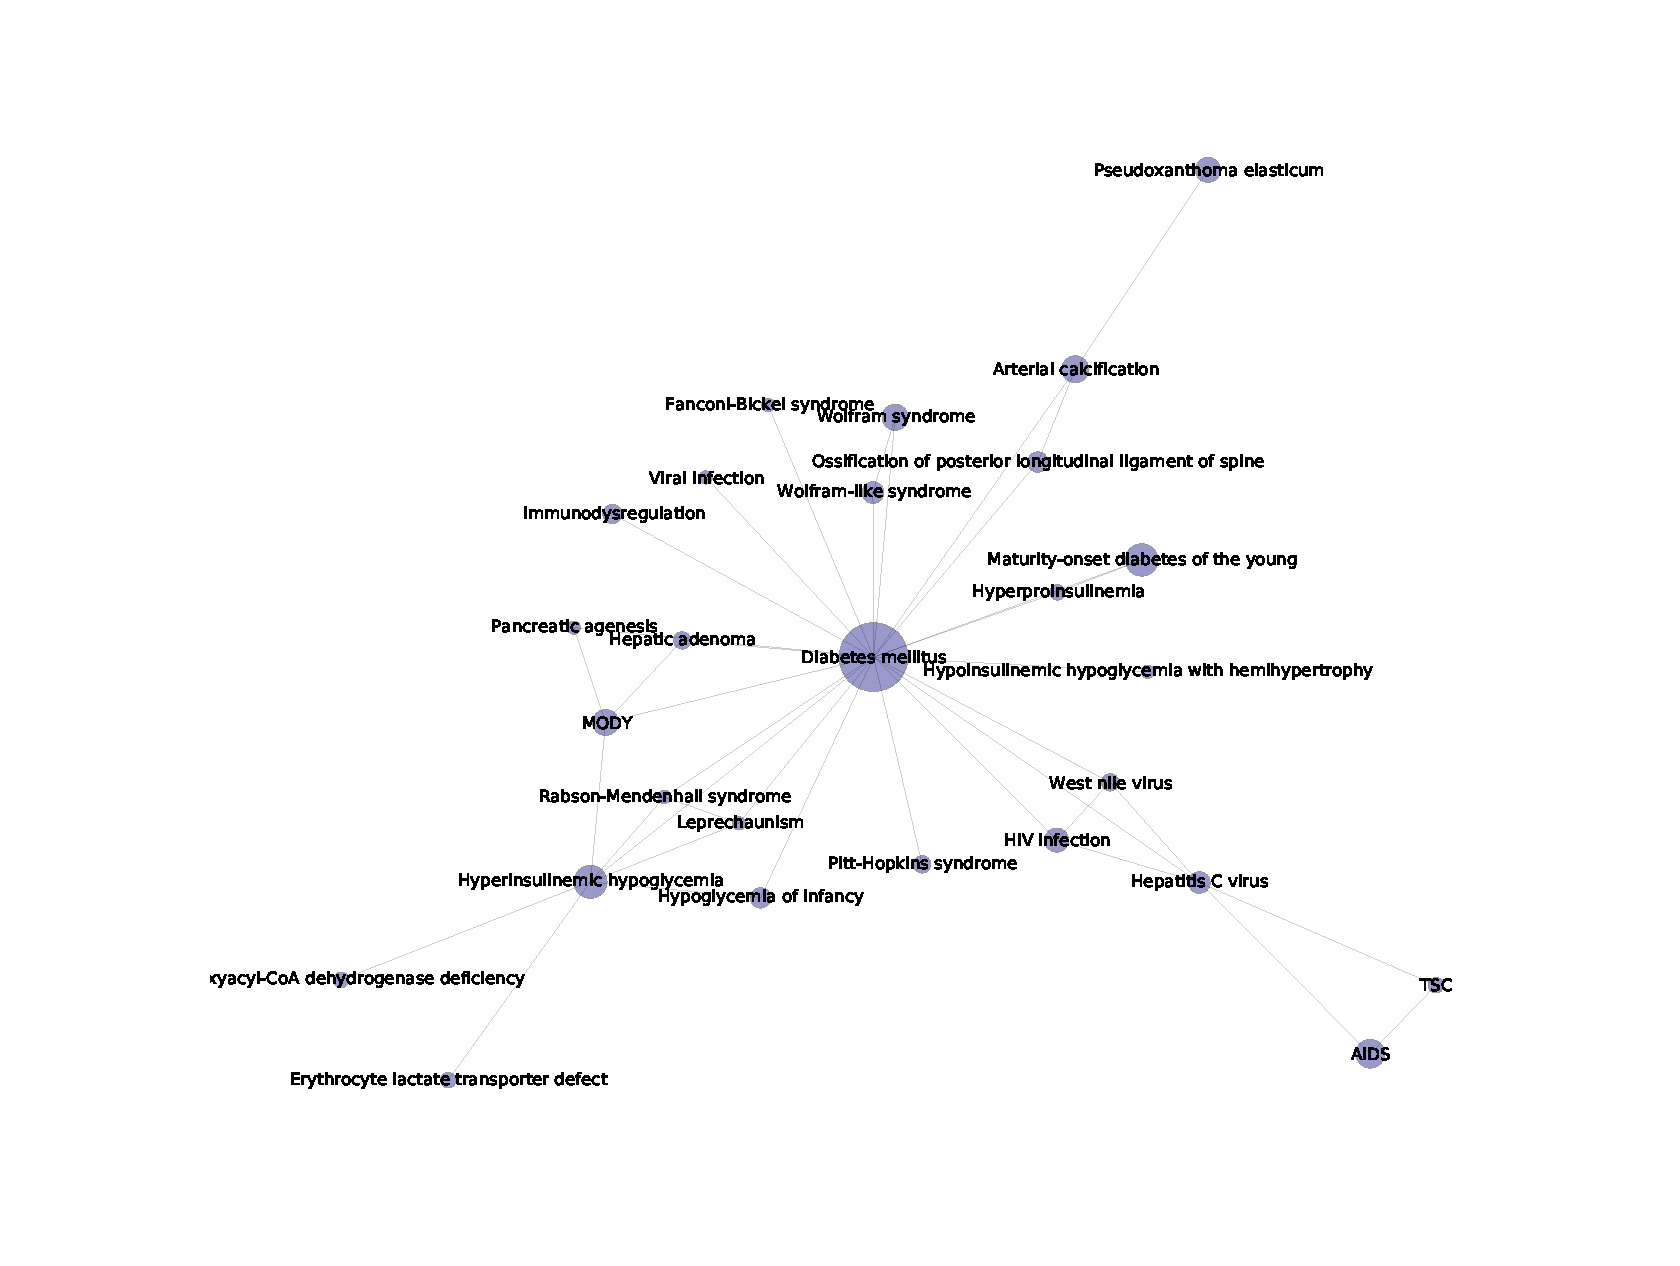
\includegraphics[scale=0.5]{img/diabetesmellitus3.pdf}
        \caption{Diabetes mellitus cluster}
        \label{diabetesmellitus3}
    \end{center}
\end{figure}


\subsection*{Honor Code}

% The following paragraph of your report should be included as is - do % not change it.

My answers to homework are my own work. I did not make solutions or code available to anyone else. I did not engage in any other activities that will dishonestly improve my results or dishonestly improve/hurt the results of others.
\begin{figure}[htbp]
    \begin{center}
        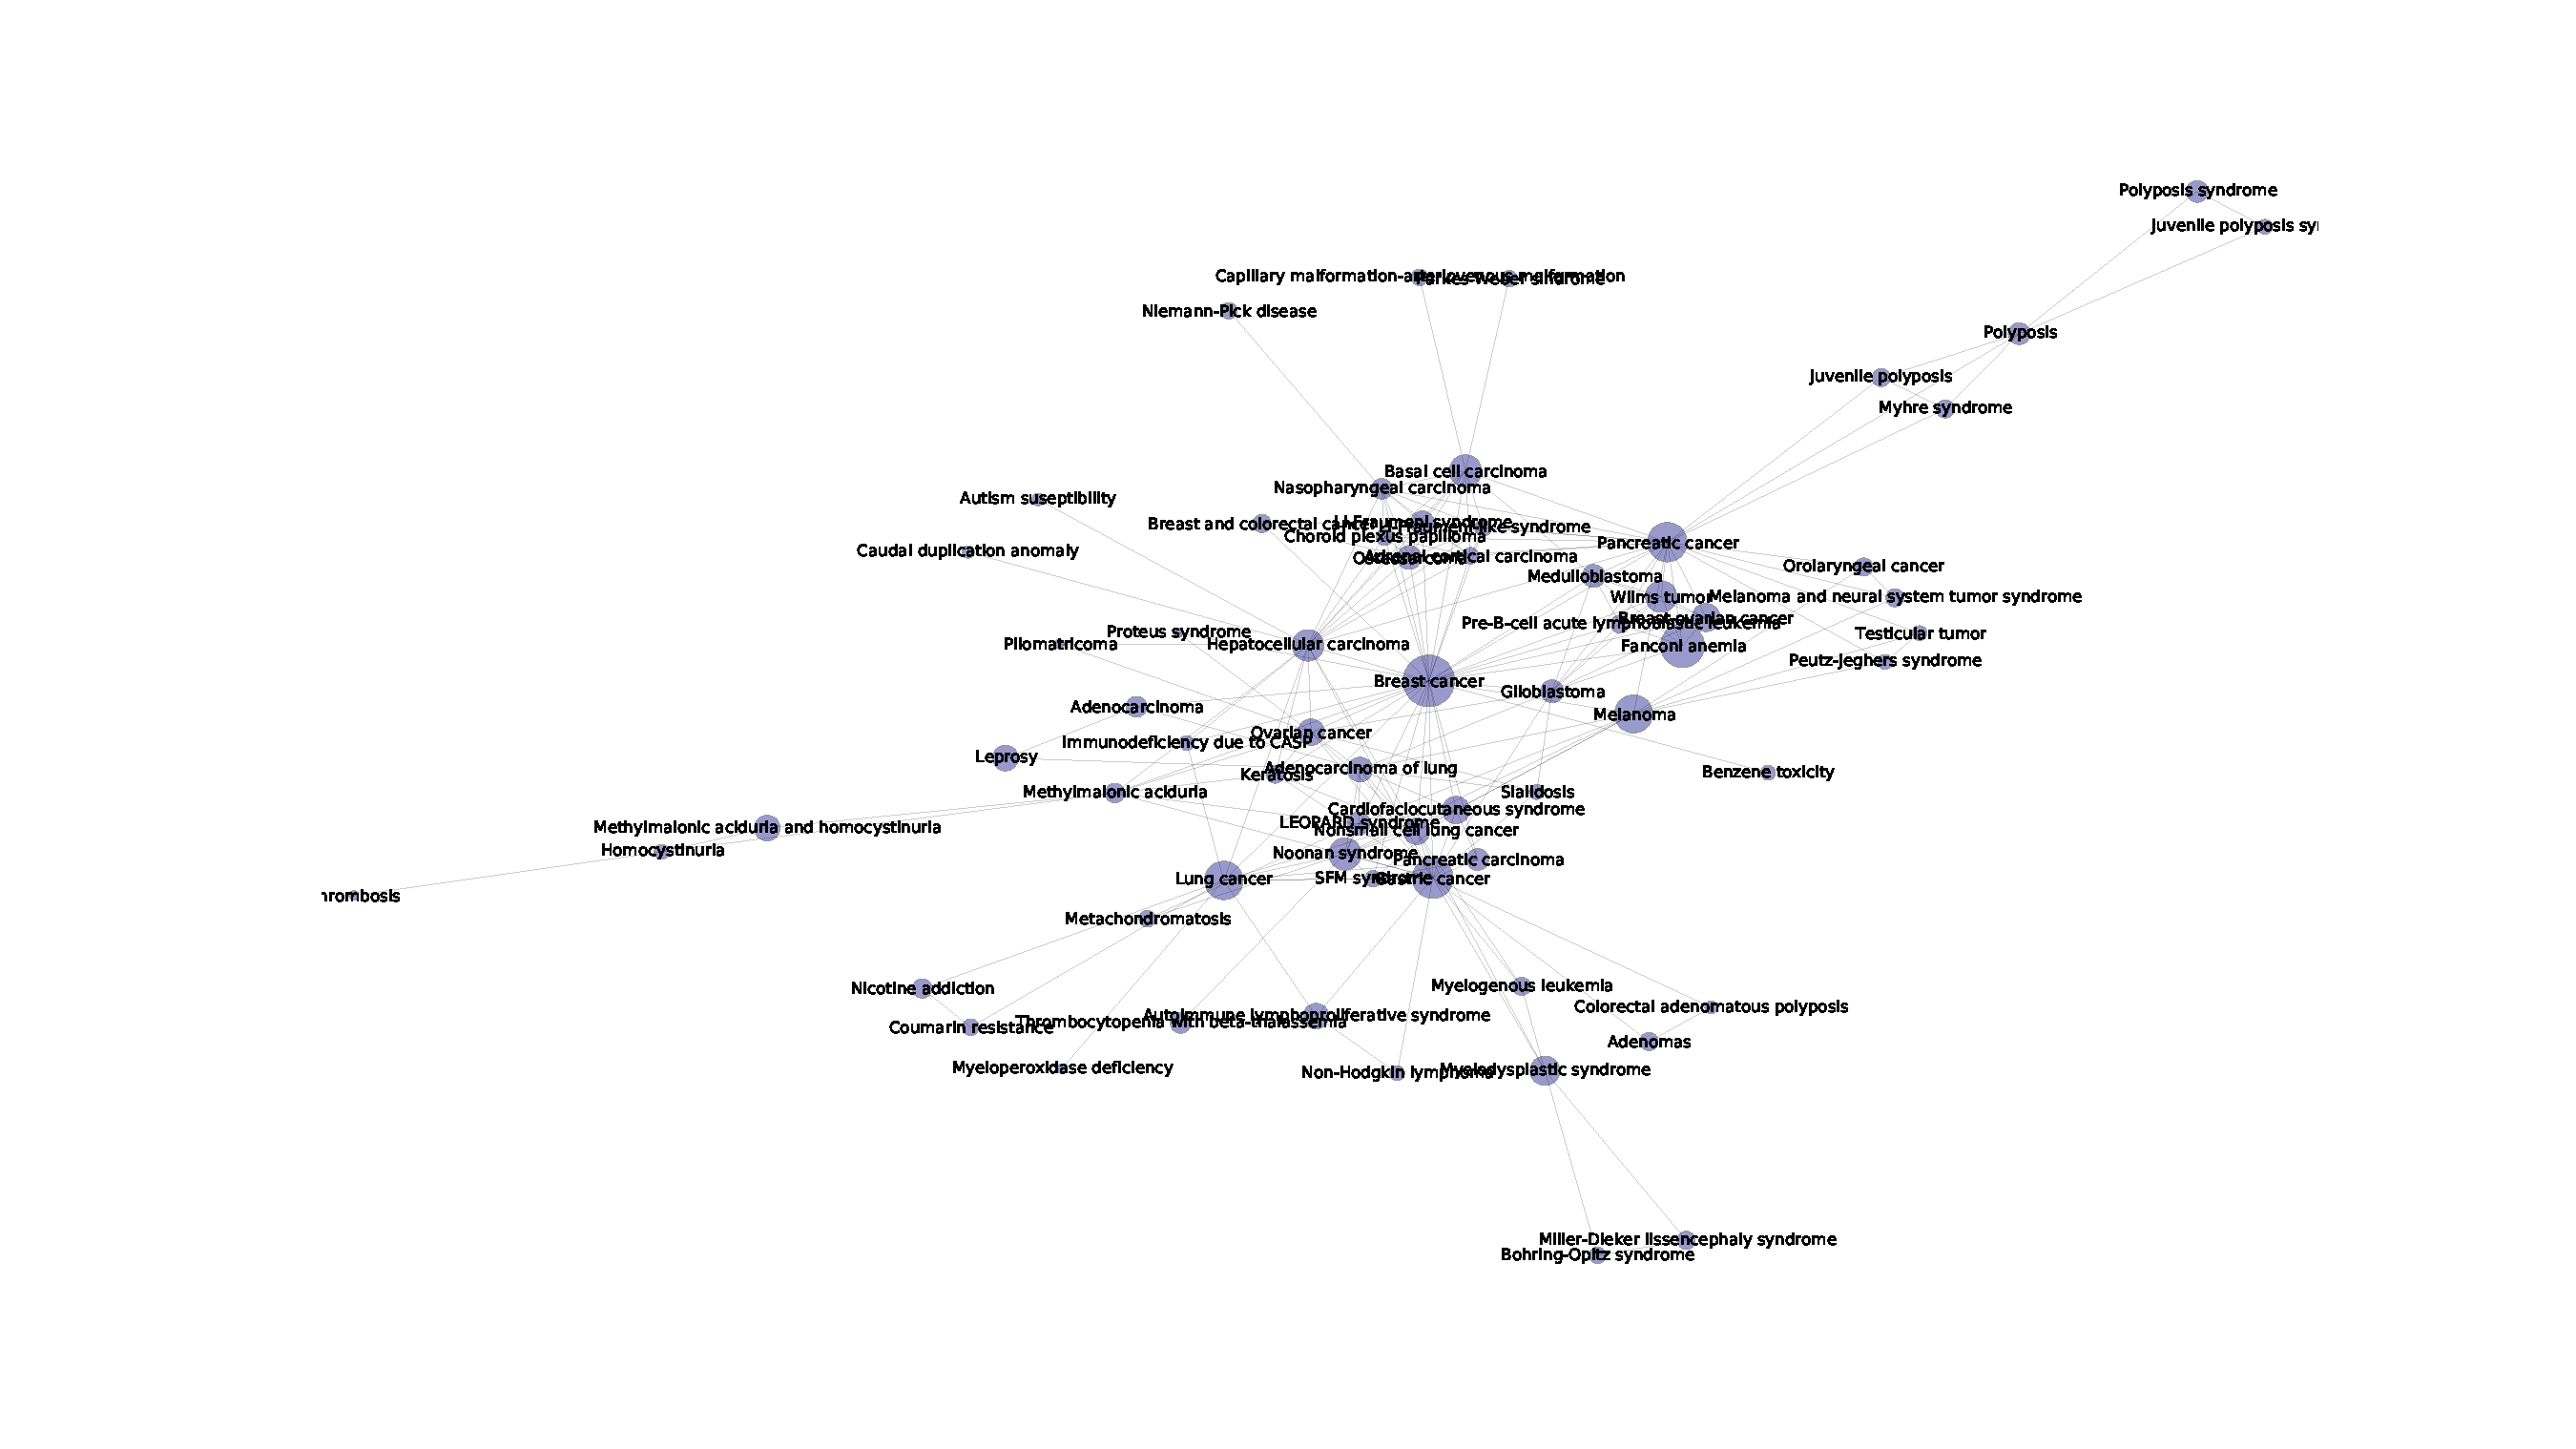
\includegraphics[scale=0.25]{img/breasCancer.pdf}
        \caption{Breast cancer cluster}
        \label{breasCancer}
    \end{center}
\end{figure}

\begin{figure}[htbp]
    \begin{center}
        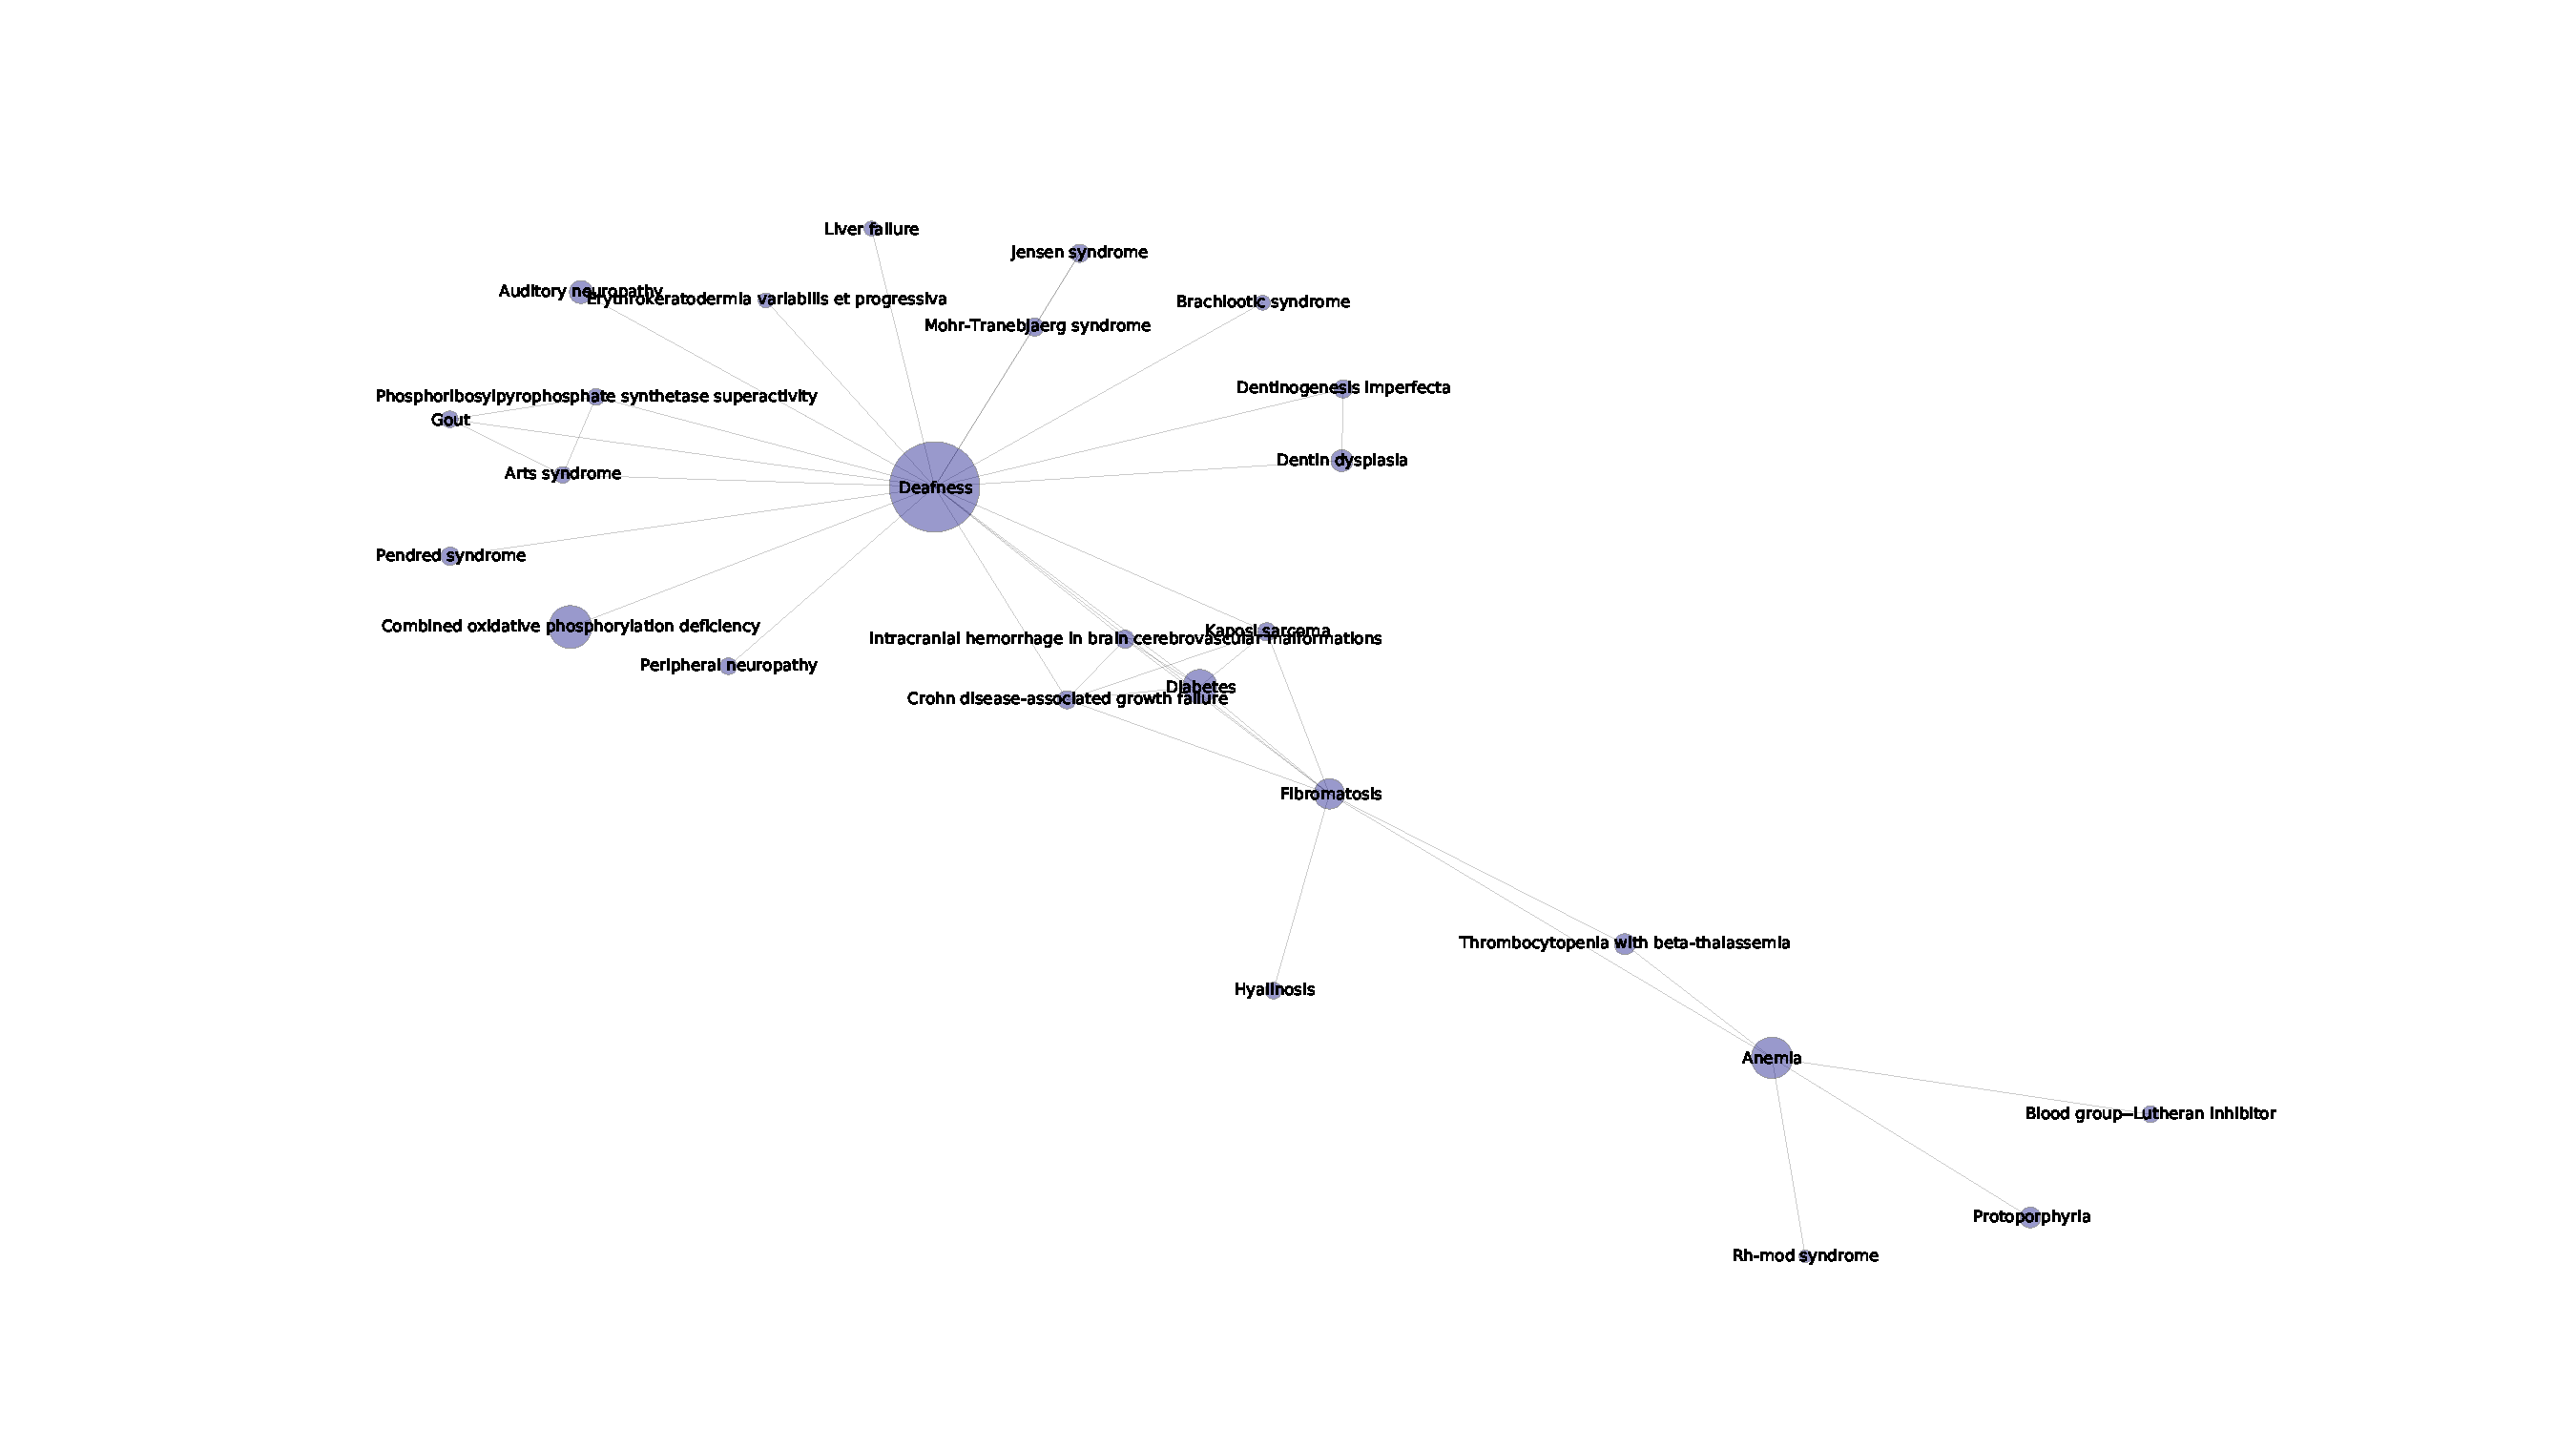
\includegraphics[scale=0.25]{img/defness.pdf}
        \caption{Deafness cluster}
        \label{defness}
    \end{center}
\end{figure}



\end{document}



%
%number of nodes:    1118
%number of edges:    3068
%number of clusters:  109
%cluster diameter:     12
%excluded connected: 1118
%
%
%Breast cancer
%number of nodes:      67
%number of edges:     205
%number of clusters:    1
%cluster diameter:      6
%
%Deafness
%number of nodes:      15
%number of edges:      17
%number of clusters:    1
%cluster diameter:      2
%
%Diabetes mellitus
%number of nodes:      30
%number of edges:      46
%number of clusters:    1
%cluster diameter:      4
%
